\section{Phase 1}
In the first phase of this project our goals were to get basic features of a scene localized in 3D space, including vehicles, lanes, pedestrians, traffic lights, and road signs. To accomplish this, we looked at different possible pipelines for the object detection and localization.

\subsection{Object Detection}
Some techniques for object detection, such as described in \emph{3D Bounding Box Estimation Using Deep Learning and Geometry} \cite{3DBoxEstimation}, will directly output a 3D bounding box of teh detected objects using a single image. These techniques have the distinct advantage of providing all needed information to render the object from a single technique, but in general the performance of these technique can be limited by the fact that are doing so much. In addition, pre-trained weights on classes other than vehicles were not easily available, and as such our team looked for other solutions.

The obvious choice, then was to use a information from multiple different networks, each providing some needed information. At the bare minimum, two networks would be needed: one to detect objects, and one to predict depth. Our team chose solutions which were easy to get running, as we wanted to focus on getting outputs from the networks as quickly as possible. To this end, we elected to use the YoloV9 framework \cite{YOLOv9}, due to its outstanding performance, and also ease of use due to the fantastic Ultralytics framework for YOLO models. The output of the YOLO model is shown in Figure \ref{fig:yolo_output}.

\begin{figure}
    \centering
    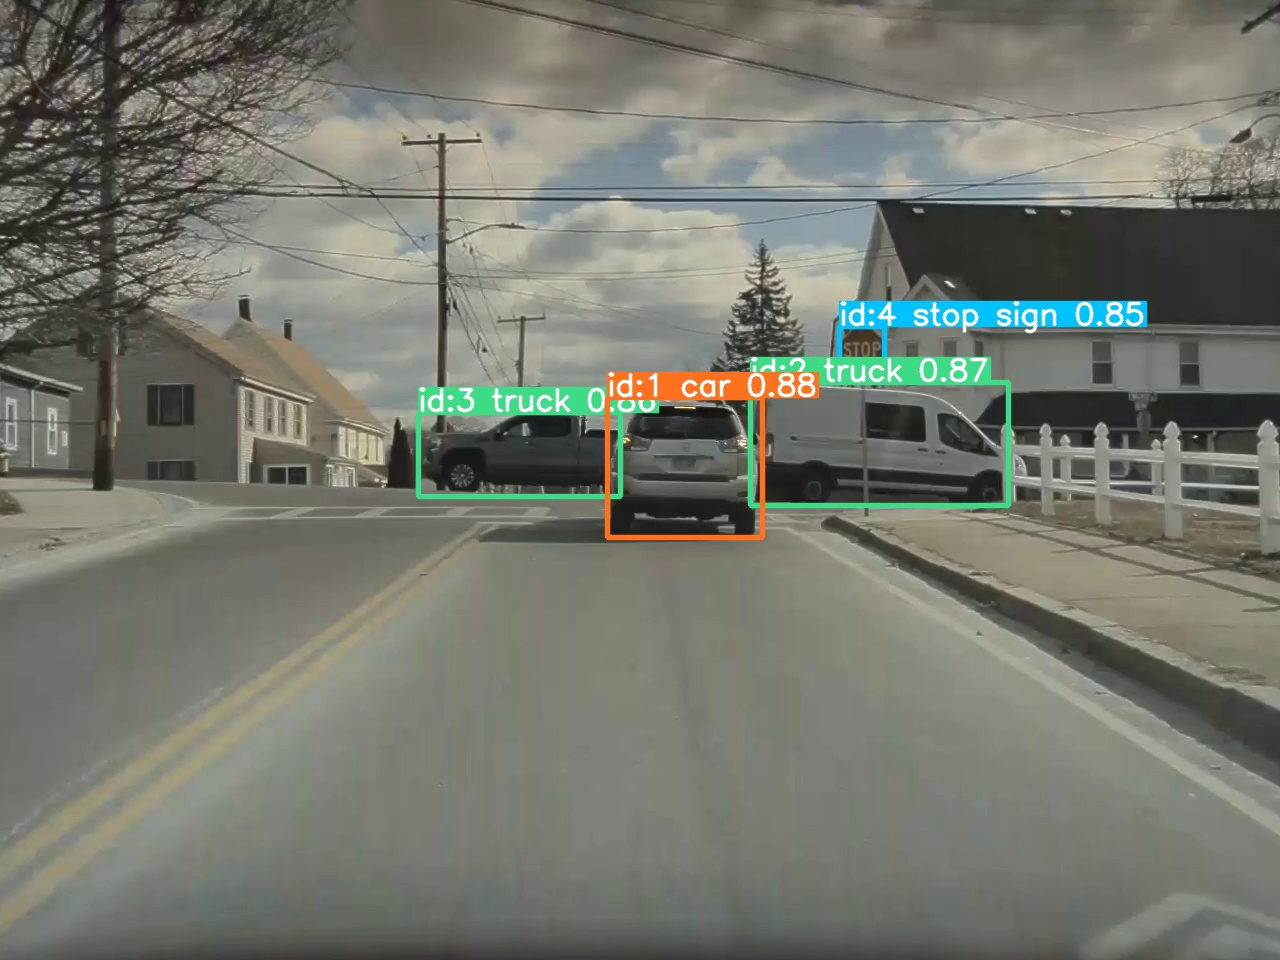
\includegraphics[width=0.95\linewidth]{images/YOLOv9.jpg}
    \caption{Output of YOLO model}
    \label{fig:yolo_output}
\end{figure}

\subsection{Depth Estimation}
For depth estimation, there are many different techniques available. One technique in particular stuck out in the early research that our team did, namely ZoeDepth \cite{ZoeDepth}. ZoeDepth is monocular metric depth estimation technique which builds upon the MiDaS architecture. The ZoeDepth model is trained on both indoor and outdoor scenes, and is able to generalize very well. ZoeDepth also had the distinct advantage of being setup to be run via TorchHub, a online repository of networks. As such, getting the network running, and integrating it into the existing YOLO pipeline was much easier. The output of the ZoeDepth model is shown in Figure \ref{fig:zoe_depth_output}.

\begin{figure}
    \centering
    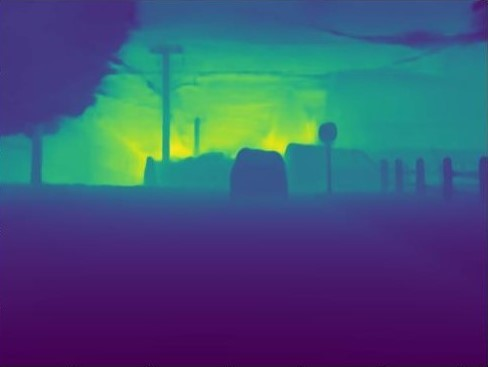
\includegraphics[width=0.95\linewidth]{images/depth.jpg}
    \caption{Output of ZoeDepth model}
    \label{fig:zoe_depth_output}
\end{figure}

\subsection{3D Localization}
Once the outputs from YOLOv9 and ZoeDepth were obtained, the next step was to localize the objects in 3D space. This was done by first taking the center of each bounding box, and then using the depth map to get the depth of the object at the center of the bounding box. The pinhole projection model was then used to get the 3D coordinates of the object.
We began with the pinhole projection model, which is shown in Equation \ref{eq:pinhole_projection}. In this equation, $\lambda$ is a scalar, $\mathbf{K}$ is the camera intrinsics matrix, $\mathbf{R}$ is the rotation matrix, $\mathbf{t}$ is the translation vector, $X$, $Y$, and $Z$ are the 3D coordinates of the object, and $x$ and $y$ are the 2D coordinates of the object in the image.
\begin{equation}\label{eq:pinhole_projection}
    \lambda\begin{bmatrix}
        x \\
        y \\
        1
    \end{bmatrix}
    =
    \mathbf{K}
    \begin{bmatrix}
        \mathbf{R} & \mathbf{t}
    \end{bmatrix}
    \begin{bmatrix}
        X \\
        Y \\
        Z \\
        1
    \end{bmatrix}
\end{equation}
The equation was then simplified by assuming $\mathbf{R}$ and $\mathbf{t}$ are the identity matrix and zero vector, respectively. This simplification is shown in Equation \ref{eq:simplified_pinhole_projection}.
\begin{equation}\label{eq:simplified_pinhole_projection}
    \lambda \mathbf{K}^{-1}\begin{bmatrix}
        x \\
        y \\
        1
    \end{bmatrix}
    =
    \begin{bmatrix}
        X \\
        Y \\
        Z
    \end{bmatrix}
\end{equation}
From this equation, we could get the ray direction of object
\begin{equation}\label{eq:ray_direction}
    \begin{bmatrix}
        X \\
        Y \\
        Z
    \end{bmatrix}
    =
    \lambda \mathbf{K}^{-1}\begin{bmatrix}
        x \\
        y \\
        1
    \end{bmatrix} 
\end{equation}
where $\lambda$ was a normalization factor, so that the magnitude of the ray direction vector was 1. The 3D coordinates of the object were then calculated by multiplying the ray direction vector by the depth of the object at the center of the bounding box, which gave the object's 3D location.

This pipeline was very effective, but it was limited by the fact that the ZoeDepth estimates the depth of the object's surface, and not the center of the object. This meant that the 3D localization was not perfect, but it was still very good. The output of the 3D localization is shown in Figure \ref{fig:3D_localization_output}.

The benefit of this pipeline is that is simple, fast, and applies for all classes of objects that the YOLO model can detect. The downside is that the 3D localization is not perfect, and no information about orientation is provided.

\subsection{3D Rendering}
Finally, to 3D render the scene, a json data-structure was created which contained the 3D coordinates and class of each detected object. This json file was then read in by a Blender python script which placed each object in the scene at the correct location. The output of the 3D rendering is shown in Figure \ref{fig:3D_localization_output}.
\begin{figure}
    \centering
    \begin{subfigure}{0.95\linewidth}
        \centering
        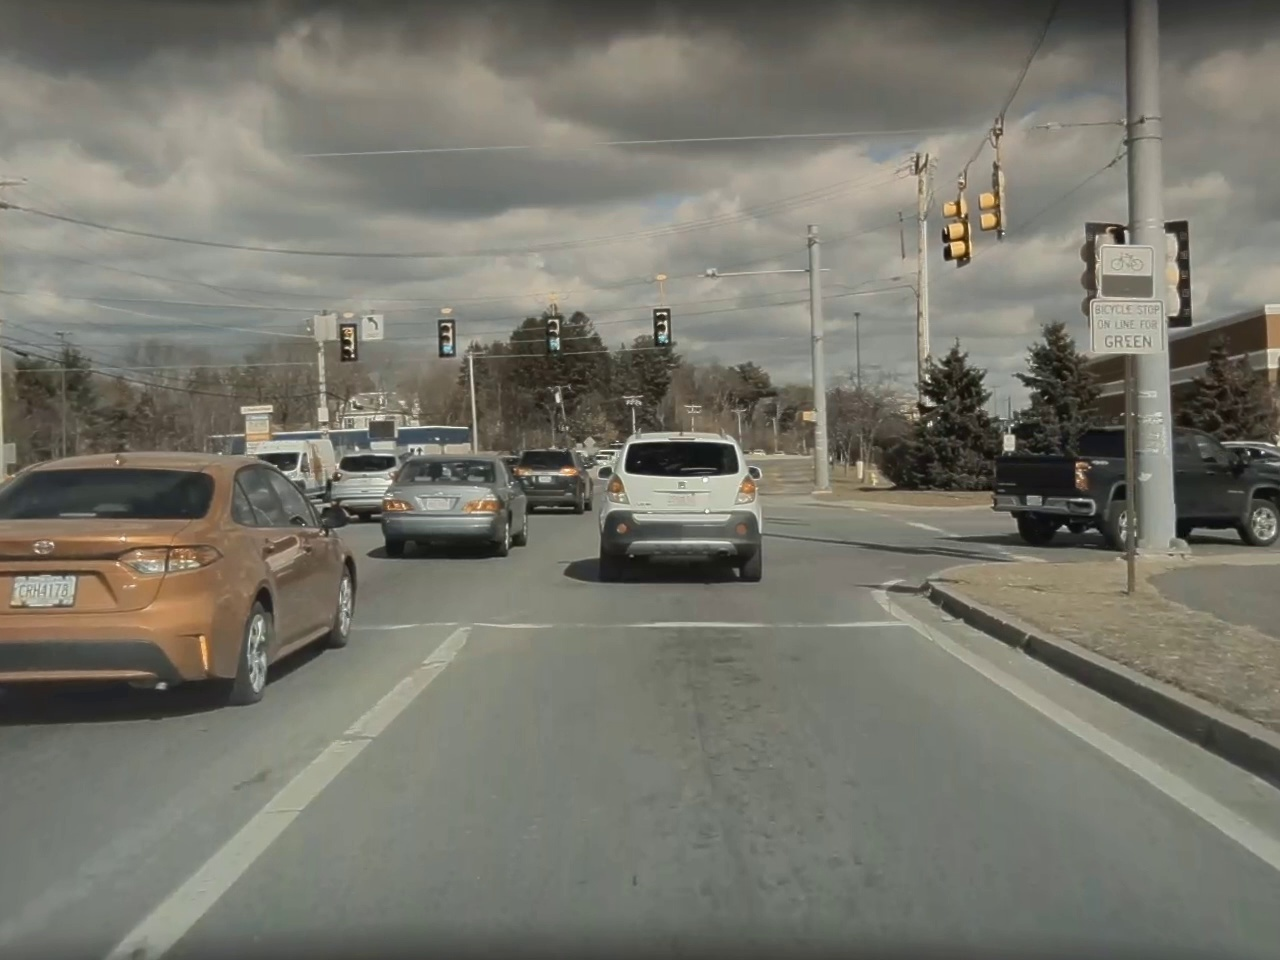
\includegraphics[width=\textwidth]{images/localization_in.jpg}
        \caption{Input image to pipeline.}
    \end{subfigure}
    \begin{subfigure}{0.95\linewidth}
        \centering
        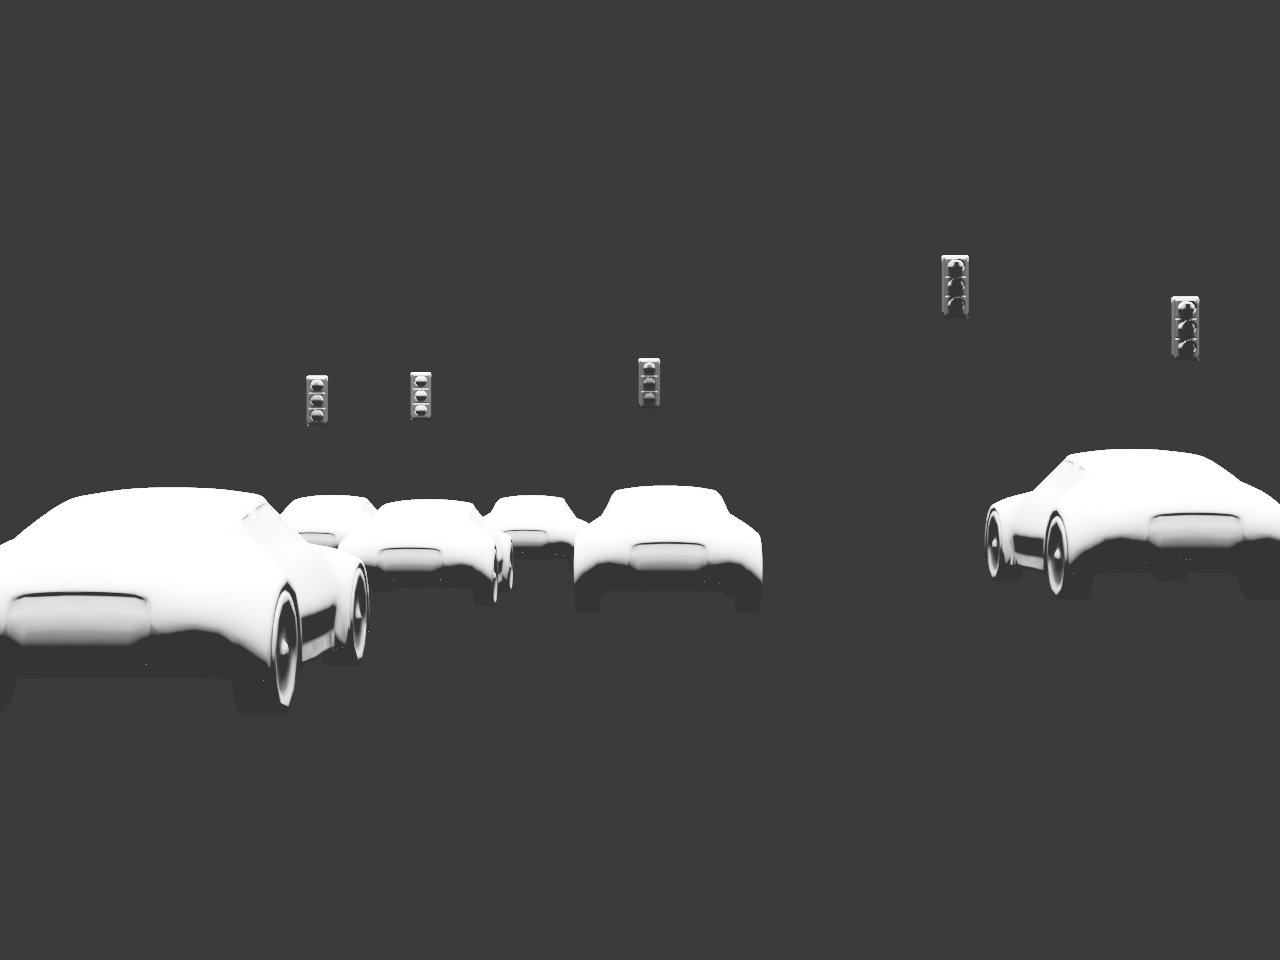
\includegraphics[width=\textwidth]{images/localization.png}
        \caption{Output of 3D localization.}
    \end{subfigure}
    \caption{3D localization of objects.}
    \label{fig:3D_localization_output}
\end{figure}

\subsection{Lane Detection}
There were many choices for lane detection, but we sought to use a technique which gave 3D lane outputs directly. We found many such powerful techniques, such as BEV-LaneDet \cite{BEV-LaneDet} and PersFormer \cite{PersFormer}, but we ran into some serious challenges with getting these networks running. In both cases, the code was publicly available on GitHub, but dependencies were not well documented, and when documented were often many years out of date, making it difficult to setup the environment to run the network. In some cases pre-trained weights were missing, making it difficult to run the test the network, or simply prohibitively expensive to train the network. In many cases, the networks were only setup to be trained and validated on datasets, and not to perform inference on new data. As a result, we were unable to get these networks running in time for the first phase of the project.

